\documentclass[11pt]{article} % Default font size is 12pt, it can be changed here
\usepackage{geometry} % Required to change the page size to A4
\geometry{a4paper} % Set the page size to be A4 as opposed to the default US Letter
\usepackage{graphicx} % Required for including pictures
\usepackage{hyperref}
\usepackage{array}
\usepackage{float} % Allows putting an [H] in \begin{figure} to specify the exact location of the figure
\usepackage{wrapfig} % Allows in-line images such as the example fish picture
\linespread{1.2} % Line spacing
\graphicspath{{./Pictures/}} % Specifies the directory where pictures are stored
\usepackage{url}

% to remove coloured boxes around the links 
\hypersetup{
    colorlinks=false,
    pdfborder={0 0 0},
}
\newenvironment{myindentpar}[1]%
 {\begin{list}{}%
         {\setlength{\leftmargin}{#1}}%
         \item[]%
 }
 {\end{list}}
%----------------------------------------------------------------------------------------
\begin{document}
%----------------------------------------------------------------------------------------
\begin{titlepage}
\newcommand{\HRule}{\rule{\linewidth}{0.5mm}} % Defines a new command for the horizontal lines, change thickness here
\center % Center everything on the page

\includegraphics{urjc} \\[0.5cm] % Include logo
\textsc{\LARGE \\Universidad Rey Juan Carlos}\\[1cm] % Name of your university/college
\textsc{\Large Master in Libre Software}\\[0.5cm] % Major heading such as course name
\HRule \\[1.5cm]
{ \huge \bfseries Case Study I}\\[0.4cm] % Title of your document
\HRule \\[1.5cm]
\begin{minipage}{0.4\textwidth}
\begin{flushleft} \large
\emph{Authors:}\\
Amal \textsc{Roumi}\\ % Your name
\end{flushleft}
\end{minipage}
%~
\begin{minipage}{0.4\textwidth}
\begin{flushright} \large
\emph{Supervisor:} \\
Gregorio  \textsc{Robles} % Supervisor's Name
\end{flushright}
\end{minipage}\\[1.5cm]
{\large \today}\\[1.8cm] % Date, change the \today to a set date if you want to be precise
\textsc CC BY-NC-SA 3.0\\[0.2cm]

\includegraphics[scale=0.5]{license} \\ % Include license
{\small http://creativecommons.org/licenses/by-nc-sa/3.0}\\
\mbox{}

\end{titlepage}


As final work for the course of “Case Studies I” that related to case II which I made before in Master of Libre software (Universidad Rey Juan Carlos), we are requested to write horizontal  report in one topic we choose in each projects that have been presented in this subject, my choice is about “History".The original work for this study can be found in  \url{https://github.com/MSWL--2013-14/mswl-csii-2014/tree/master/Amal-History}.

\section{History of Free and Open Source Software}

Long time in the early 1950's before the term “Open Source” was used, software was developed by loose associations of programmers and freely exchanged. Organizations such as SHARE and DECUS developed much of the software that computer hardware companies bundled with their hardware offerings. At that time computer companies were in the hardware business; anything that reduced software cost and made more programs available made the hardware companies more competitive.
\paragraph{Successes for Free Software}

In 1983, Richard Stallman launched the GNU Project to write a complete operating system.
 free from constraints on use of its source code. Stallman also published the GNU Manifesto, in 1985, to outline the GNU project's purpose and explain the importance of free software. Soon after the launch, he coined the term "free software" and founded the Free Software Foundation to promote the concept and a free software definition
  \footnote
 {The definition had two points:
\begin{enumerate}
 \item "The word "free" in our name does not refer to price; it refers to freedom. First, the freedom to copy a program and redistribute it to your neighbors, so that they can use it as well as you. Second, the freedom to change a program, so that you can control it instead of it controlling you; for this, the source code must be made available to you."
  \item Four freedom
\begin{itemize}
\item The freedom to run the program, for any purpose (freedom 0).
\item The freedom to study how the program works, and change it so it does your computing as you wish (freedom 1). Access to the source code is a precondition for this.
\item The freedom to redistribute copies so you can help your neighbour (freedom 2).
\item The freedom to distribute copies of your modified versions to others (freedom 3). By doing this you can give the whole community a chance to benefit from your changes. Access to the source code is a precondition for this.
\end{itemize} 
\end{enumerate}
}
 was published in February 1986. In 1989, the first version of the GNU General Public License was published. A slightly updated version 2 was published in 1991.

\paragraph{Linux}
 The Linux kernel, started by Linus Torvalds, was released as freely modifiable source code in 1991. The licence wasn't a free-software licence, but with version 0.12 in February 1992, Torvalds relicensed the project under the GNU General Public License.
Until this point, the GNU project's lack of a kernel meant that no complete free-software operating systems existed. \\The combination of the almost-finished GNU operating system and the Linux kernel made the first complete free-software operating system. Among Linux distributions, Debian GNU/Linux, begun by Ian Murdock in 1993.
\paragraph{Open Source}
In 1997, Eric Raymond published The Cathedral and the Bazaar, a reflective analysis of the hacker community and free-software principles. The paper received significant attention in early 1998 and was one factor in motivating Netscape Communications Corporation to release their popular Netscape Communicator Internet suite as free software. 
In February 1998, Raymond made the first public call to the free software community to adopt the new term. The Open Source Initiative \footnote{\url{http://opensource.org/}} was formed shortly thereafter by Eric Raymond and Bruce Perens.\\
Starting in the beginning of the 2000s, a number of companies began to publish a small parts of their source code to claim they were open source, while keeping key parts closed. This led to the development of the now widely used terms free open-source software and commercial open-source software to distinguish between truly open and hybrid forms of open source.

\section{Briefs about each project and their history}
%------------------------------------------------
\subsection{FreeBSD Project }
 Homepage :\url {https://www.freebsd.org/}\\

\subparagraph{What is the Free BSD}

FreeBSD is an operating system for desktops, laptops, servers, and embedded systems with support for a large number of platforms. which focuses on features, speed, and stability. It is derived from BSD, the version of UNIX developed at the University of California, Berkeley. It is developed and maintained by a large community.\\

\textit{The differences between FreeBSD and NetBSD, OpenBSD}
\begin{itemize}
\item OpenBSD aims for operating system security above all else. The OpenBSD team wrote ssh \footnote{\url {http://www.freebsd.org/cgi/man.cgi?query=ssh&sektion=1}} and pf \footnote{\url{http://www.freebsd.org/cgi/man.cgi?query=pf&sektion=4}}, which have both been ported to FreeBSD.
\item NetBSD aims to be easily ported to other hardware platforms.
\item  DragonFly BSD is a fork of FreeBSD 4.8 that has since developed many interesting features of its own, including the HAMMER file system and support for user-mode “vkernels”.
\end{itemize}
       \begin{figure}
   \centering
        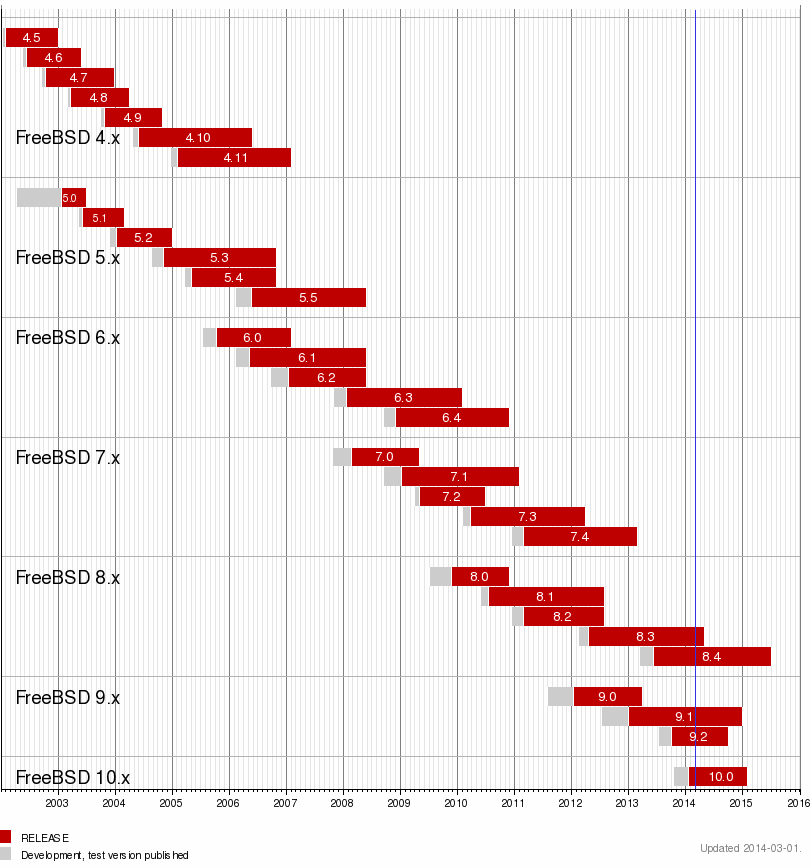
\includegraphics[scale=0.4]{./freebsd.png}
     \caption{ The time line shows that the span of a single release generation of FreeBSD lasts around 5 years.}
      \end{figure}


  \subparagraph{History and Timeline} \mbox{} \\
The FreeBSD Project had its genesis in the early part of 1993, partially as an outgrowth of the Unofficial 386BSD Patchkit by the patchkit's last 3 coordinators: Nate Williams, Rod Grimes and Jordan Hubbard.

The first distribution was FreeBSD 1.0, released in December of 1993. This was based on the 4.3BSD-Lite (“Net/2”) tape from U.C. Berkeley, with many components also provided by 386BSD and the Free Software Foundation. It was a fairly reasonable success for a first offering, and they followed it with the highly successful FreeBSD 1.1 release in 1994.
 After a lawsuit between then Unix copyright owner Unix System Laboratories, and the University of California, Berkeley, the FreeBSD project re-engineered most of the system using the 4.4BSD-Lite release from Berkeley, which, owing to the lawsuit, had none of the AT\&T source code earlier BSD versions contained, making it an un bootable operating system. Following much work, the unencumbered outcome was released as FreeBSD 2.0 in January 1995.
Since that time, FreeBSD has made a series of releases each time improving the stability, speed, and feature set of the previous version.\\
In the following image shows the time line that the span of a single release generation of FreeBSD lasts around 5 years
\pagebreak


\subsection{Mercurial}
Webpage \url{http://mercurial.selenic.com/}\\
Mercurial is a cross-platform, distributed revision control tool for software developers. It is mainly implemented using the Python programming language, but includes a binary diff implementation written in C. It is supported on MS Windows and Unix-like systems, such as FreeBSD, Mac OS X and Linux. Mercurial is primarily a command line program but graphical user interface extensions are available. All of Mercurial's operations are invoked as arguments to its driver program hg, a reference to the chemical symbol of the element mercury.\footnote{http://en.wikipedia.org/wiki/Mercurial}

  \subparagraph{History and Time-line} \mbox{} \\
    First announced Mercurial on 19 April 2005 by Mackall. The impetus for this was the announcement earlier that month by Bitmover that they were withdrawing the free version of BitKeeper. Mackall decided to write a distributed VCS as a replacement for use with the Linux kernel.
Mercurial started after the project {\bf Gi}t which is initiated by Linus Torvalds with similar aims.\footnote{ The goals:\url{http://lkml.iu.edu//hypermail/linux/kernel/0504.2/0670.html}
\begin{itemize}
\item - to initially be as simple (and thereby hackable) as possible

\item- to be as scalable as possible.

\item- to be memory, disk, and bandwidth efficient.

\item- to be able to do "clone/branch and pull/sync" style development. \end{itemize}
}
The Linux kernel project decided to use Git rather than Mercurial, but Mercurial is now used by many other projects .

%==============================================================

\subsection{SilverStripe CMS} 
Webpage \url{http://www.silverstripe.com/}\\
   SilverStripe is a free and open source Content Management System (CMS) and Framework for creating and maintaining websites and web applications. It provides an out of the box web-based administration panel that enables users to make modifications to parts of the website, which includes a WYSIWYG \footnote{ An acronym for "What You See Is What You Get"}website editor. The core of the software is SilverStripe Framework, a PHP Web application framework.
  
  \subparagraph{History and Time-line}\footnote{http://www.silverstripe.org/our-history/}
\begin{itemize}
\item SilverStripe Ltd. was founded in 2000 in Wellington, New Zealand, by Tim Copeland, Sam Minnée, and Sigurd Magnusson. The three originally developed and marketed a closed-source PHP4-based CMS to local small and medium-sized business customers.later they have grown from three staff to over 40.
\item In late 2005, the business decided to rebuild this CMS from scratch in PHP5,
\item In 2006: SilverStripe CMS became a member of Wellington’s Creative HQ business incubator.
\item SilverStripe 2.0 released in 2007 publicly as free and open source software under BSD license.The project was accepted into the Google Summer of Code, one of only 16 software projects to do so.
\item In late 2008, SilverStripe split its main website into silverstripe.com, to act as the home for the company behind the software, and silverstripe.org, to act as the home for the software and its open source community.
\item SilverStripe in 2010, claimed the software had been downloaded 250,000 times since first released.
\item In 2010, CMS gained Microsoft SQL Server support, and became the first open source web application to become Microsoft Certified. Due to popular demand from the community, two books on SilverStripe CMS were released: one in German, and one in English.

\item SilverStripe 3.0 CMS released in 2012, containing significant usability and developer API changes; SilverStripe Framework was released for the first time as a stand-alone framework.
\item SilverStripe CMS 3.1,released in 2013 , with more visual feedback and easier preview, composer support, YAML configuration and an improved UploadFeild


\end{itemize}
%==============================================================

\subsection{Camino}
Webpage \url{http://caminobrowser.org/}\\
 \textbf{Camino} is Spanish, as in \textbf{el Camino}. It means “way” or “path” and is an extension of the “Navigator” idea from which this project originally sprang.\\
 Camino is a free, open-source web browser for Mac OS X. It uses Apple’s Cocoa programming toolkit and the Gecko web page rendering engine from Mozilla.Camino is developed by the volunteer members of the Camino Project.
and evolved from being a side project of Mozilla into a fully fledged open source browser for Mac.\\
\textbf{ The difference between Camino and Firefox.} \\
 Camino is a native Mac OS X application; this means it will only work on the Mac platform. Firefox, however, works on several operating systems.
  \subparagraph{History and Time-line} \mbox{} \\
Camino started with some work back in late 2001 that \textit{Vidur Apparao} and \textit{Mike Pinkerton} to prove that they could embed Gecko in a Cocoa application. 
 In early 2002 Dave Hyatt, one of the co-creators of Firefox , joined the team and built Chimera, a small, lightweight browser wrapper, around their work.
       \begin{figure}
   \centering
        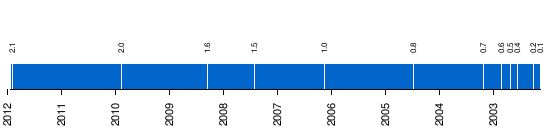
\includegraphics[scale=0.6]{./Caminotimeline.png}
     \caption{Camino Time-line}
      \end{figure}
  \begin{itemize}
  
 \item Chimera 0.1 the first downloadable was released in 2002, the early releases became popular due to their fast page-loading speeds (as compared with then-dominant Mac browser, Microsoft's Internet Explorer version 5).
 \item In mid-2002 Hyatt was hired by Apple Computer to start work on what would become Safari. 
 \item The Chimera developers got a small team together within Netscape, with dedicated development and QA, to put together a Netscape-branded technology preview.
 \item Name was changed from Chimera to Camino for legal reasons.
 \item Camino 0.7 ,released in 2003 was primarily a Netscape-driven release kept afloat at the end by open source.
  \item Camino 0.8 ,released in 2004 was according to Pinkerton "a triumph of open source and open process. People from all around the world helped with patches, QA, bug triage, localization, artwork, and evangelism."\footnote{http://arstechnica.com/apple/2004/09/mac-20040923/}\\
 \item In 2005, Camino's Web site was moved from the Mozilla Foundation's domain mozilla.org to the Camino Project's domain caminobrowser.org.
 \item In 2005, Pinkerton accepted a position at Google where he worked closely with Google's Firefox team and continued to work on Camino.
 \item Camino 1.0 ,released in 2006,was the first browser of the Mozilla family to appear as a universal binary.
 \item Camino 2.0 ,released in 2009, It was the first Camino release to be Acid2-compliant.
 \item Camino 2.1 ,released in 2011, the developers announced plans to transition to WebKit for future versions, as Mozilla had dropped support for Gecko embedding.
 \item Camino 2.1.2 released in 2012 and the final release.
\item On May 30, 2013, Stuart Morgan announced on Camino Blog that Camino has reached its end and is no longer being developed. \footnote{http://caminobrowser.org/blog/2013/}.
 \end{itemize}

%==============================================================

\subsection{Linux Kernel}

Webpage \url{https://www.kernel.org/}\\
\textbf{What is Linux?}\\Linux is a clone of the operating system Unix, written from scratch by Linus Torvalds with assistance from a loosely-knit team of hackers across the Net. It aims towards POSIX and Single UNIX Specification compliance.
The Linux Kernel Organization is a California Public Benefit Corporation established in 2002 to distribute the Linux kernel and other Open Source software to the public without charge.released under GNU GPL version 2 and is therefore Free Software as defined by the Free Software Foundation.
  \subparagraph{History and Time-line}\footnote{\url{http://www.ragibhasan.com/linux}}
The History of Linux began in 1991 with the commencement of a personal project by a Finnish student, Linus Torvalds, to create a new free operating system kernel.

Since then, the resulting Linux kernel has been marked by constant growth throughout its history. Since the initial release of its source code in 1991, it has grown from a small number of C files under a license prohibiting commercial distribution to the 3.10 version in 2013 with more than 16 million lines of source code under the GNU General Public License.
\begin{itemize}
\item In 1984 Richard Stallman quits his job at MIT and starts working on the GNU Project.
\item Free Software Foundation, an organization for creating and promoting free software, is founded by Richard Stallman in 1985.
\item The GNU manifesto, a statement by Richard Stallman advocating the cause of free software movement, is published in the March 1985 issue of Dr. Dobb's Journal

\item
In 1991 	Linus conceives the idea of Linux and announces the project in a Usenet Post and Version 0.01 is released on the Net
\item In 1992 	First Linux Newsgroup: alt.os.linux founded in the UseNet
, Ari Lemmke starts the popular Linux newsgroup comp.os.linux in the UseNet
,Adam Richter announces the release of the first Linux Distribution from his company: Yggdrasil

\item Slackware, the famous Linux distribution is released by Peter Volkerding , and Matt Welsh releases Linux Installation getting started: version 1 in 1993
\item Linux kernel version 1.0 is released in 1994
\item Linux kernel Version 2.0 released in 1996.
\item Linux kernel Version 3.0 released in 2011.

\item In 2013 Google's Linux-based Android claims 75\% of the smartphone market share, in terms of the number of phones shipped.
\end{itemize}


        \begin{figure}
   \centering
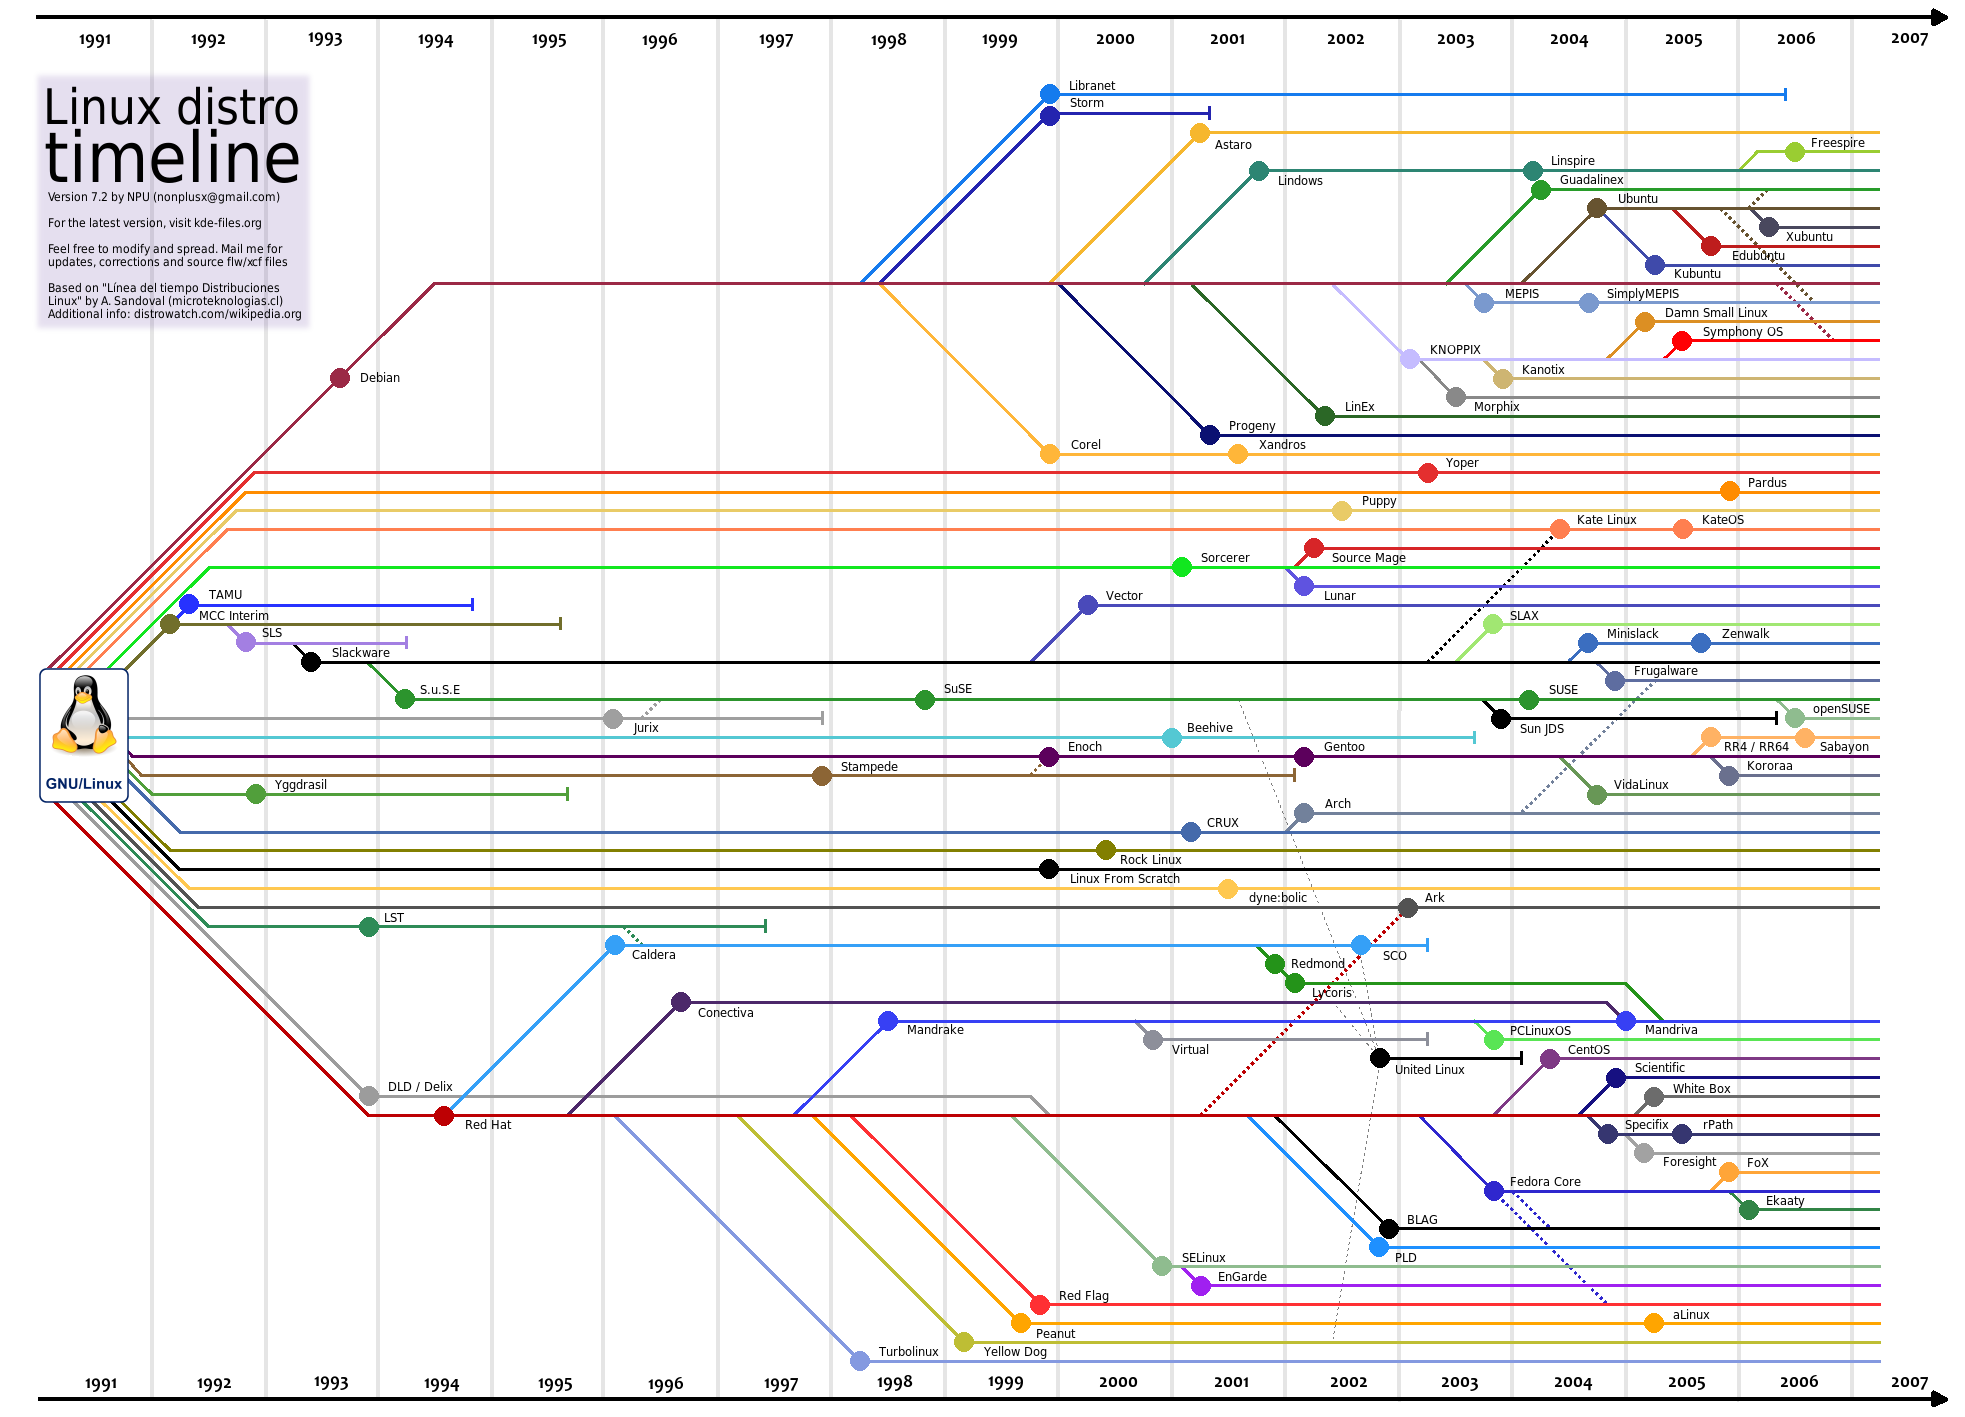
\includegraphics[scale=0.2]{linuxdistrotimeline.png}
\caption{{\tiny Source :\url{http://www.cyberciti.biz/tips/wp-content/uploads/2007/06/44218-linuxdistrotimeline-7.2.png}}}
      \end{figure}




\newpage
%==============================================================

\newpage 
%  table of contents
%----------------------------------------------------------------------------------------
\tableofcontents
\newpage
%================================================================================

%----------------------------------------------------------------------------------------
%	 BIBLIOGRAPHY
%----------------------------------------------------------------------------------------
  \begin{thebibliography}{1}

  \bibitem{notes}{History of Free and Open Source Software}\\ \url{http://en.wikipedia.org/wiki/History_of_free_and_open_source_software}.
  
   \bibitem{notes} Timeline of OpenBSD\\ \url{ http://en.wikipedia.org/wiki/OpenBSD_timeline}
   \bibitem{notes} Eric Bangeman - 2004 {Interview with Camino Project head Mike Pinkerton}\\        \url{http://arstechnica.com/apple/2004/09/mac-20040923/}
   \bibitem{notes} Free BSD webpage \\ \url {https://www.freebsd.org/}.
    \bibitem {notes} mercurial webpage \url{http://mercurial.selenic.com/}.
   \bibitem{notes}SilverStripe webpage \\\url{http://www.silverstripe.com/}.
   \bibitem{notes}Camino webpage\\  \url{http://caminobrowser.org/}

   \bibitem{notes}Linux Kernel webpage \\ \url{https://www.kernel.org/}
   \bibitem {notes}\url{http://en.wikipedia.org/wiki/History_of_the_Linux_kernel}
   \bibitem{notes} \url {http://kernelnewbies.org/LinuxChanges}
      \bibitem{notes} History of Linux by Ragib Hasan\\ \url {http://www.ragibhasan.com/linux/}
   \bibitem{notes}Changes done in each Linux kernel release\\ \url {http://kernelnewbies.org/LinuxChanges}
      \bibitem{notes}  LINUX's History by Linus Torvalds\\ \url {http://www.cs.cmu.edu/~awb/linux.history.html}
 \bibitem{notes}How the FreeBSD Project Works\\ \url{http://www.youtube.com/watch?v=nNkqKdLm1rU}
 \bibitem{notes} SilverStripe CMS\\ \url{http://www.youtube.com/watch?v=9hHHfNJAvi8}
 \bibitem{notes}Camino\\ \url{http://www.youtube.com/watch?v=vGTbVz38CNo}
 \bibitem{notes} Greg Kroah Hartman on the Linux Kernel\\ \url{http://www.youtube.com/watch?v=L2SED6sewRw}
 \bibitem{notes} Mercurial Project \\\url {http://www.youtube.com/watch?v=1sV8Z_Lmpt4}
 
  \end {thebibliography}

\end{document}
